\documentclass[10pt]{article}
\usepackage{kotex}
\usepackage{enumerate}
\usepackage{commath}

% Packages for formatting
\usepackage[margin=1in]{geometry}
\usepackage{fancyhdr}
\usepackage{graphicx}
\usepackage{amsmath}
\usepackage{amsthm}
\usepackage{algorithm2e,setspace}
\usepackage{algpseudocode}
\usepackage{xcolor}
\usepackage{amssymb}

% Fonts
\usepackage[T1]{fontenc}
\usepackage[utf8]{inputenc}
\usepackage{newpxtext,newpxmath}
\usepackage{sectsty}

% Define colors
\definecolor{blue1}{HTML}{0077c2}
\definecolor{blue2}{HTML}{00a5e6}
\definecolor{blue3}{HTML}{b3e0ff}
\definecolor{blue4}{HTML}{00293c}
\definecolor{blue5}{HTML}{e6f7ff}

\definecolor{thmcolor}{RGB}{231, 76, 60}
\definecolor{defcolor}{RGB}{52, 152, 219}
\definecolor{lemcolor}{RGB}{155, 89, 182}
\definecolor{corcolor}{RGB}{46, 204, 113}
\definecolor{procolor}{RGB}{241, 196, 15}

\usepackage{color,soul}
\usepackage{soul}
\newcommand{\mathcolorbox}[2]{\colorbox{#1}{$\displaystyle #2$}}
\usepackage{cancel}
\newcommand\crossout[3][black]{\renewcommand\CancelColor{\color{#1}}\cancelto{#2}{#3}}
\newcommand\ncrossout[2][black]{\renewcommand\CancelColor{\color{#1}}\cancel{#2}}

\usepackage{hyperref}

% Chapter formatting
\definecolor{titleblue}{RGB}{0,53,128}
\usepackage{titlesec}
\titleformat{\section}
{\normalfont\sffamily\Large\bfseries\color{titleblue!100!gray}}{\thesection}{1em}{}
\titleformat{\subsection}
{\normalfont\sffamily\large\bfseries\color{titleblue!75!gray}}{\thesubsection}{1em}{}
\titleformat{\subsubsection}
{\normalfont\sffamily\normalsize\bfseries\color{titleblue!50!gray}}{\thesubsubsection}{1em}{}


%Tcolorbox
\usepackage[most]{tcolorbox}

%Tikzpicture
\usepackage{tikz}
\usetikzlibrary{shapes,arrows,positioning}
\usepackage{tikz-cd}
\usetikzlibrary{positioning}

\usepackage{tocloft}

% Header and footer formatting
\pagestyle{fancy}
\fancyhead{}
\fancyhf{}
\rhead{Student ID: 20192250\quad Name: 지용현}%\rule{3cm}{0.4pt}}
\lhead{\textcolor{blue2}{\textbf{고급응용수학 과제 \#1}}}
% Define footer
\newcommand{\footer}[1]{
\begin{flushright}
\vspace{2em}

\includegraphics[width=2cm]{school_logo.jpg} \\
\vspace{1em}
\textcolor{blue2}{\small\textbf{#1}}
\end{flushright}
}
%\rfoot{\large Department of Information Security, Cryptogrphy and Mathematics, Kookmin Uni.
\includegraphics[height=1.5cm]{school_logo.jpg}}
\fancyfoot{}
\fancyfoot[C]{-\thepage-}


%Listing
\usepackage{listings} %Code
\renewcommand{\lstlistingname}{Code}%

\definecolor{sagegreen}{rgb}{0.0,0.6,0.4}
\definecolor{sagepurple}{rgb}{0.6,0.0,0.4}
\definecolor{sageblue}{rgb}{0.0,0.4,0.6}
\definecolor{sageorange}{rgb}{1.0,0.4,0.0}
\definecolor{sagegray}{rgb}{0.4,0.4,0.4}

\lstdefinestyle{sage}{
language=Python,
backgroundcolor=\color{white},
basicstyle=\small\ttfamily\color{black}, 
basicstyle=\footnotesize\ttfamily\color{black},
keywordstyle=\color{blue!60!black},
commentstyle=\color{green!60!black},
stringstyle=\color{purple!60!black},
showstringspaces=false,
breaklines=true,
tabsize=4,
morekeywords={True, False, None},
frame=leftline, % Remove the border
framesep=3pt,
frameround=tttt,
framexleftmargin=3pt,
numbers=left,
numberstyle=\small\color{gray},
xleftmargin=15pt, % Increase the left margin
xrightmargin=5pt,
captionpos=b,
belowskip=0pt,
aboveskip=4pt
}

\usepackage{amsthm}
\newtheorem{axiom}{Axiom}[section]
\newtheorem{theorem}{Theorem}
\newtheorem*{theorem*}{Theorem}
\newtheorem{proposition}[theorem]{Proposition}
\newtheorem{corollary}{Corollary}[theorem]
\newtheorem*{corollary*}{Corollary}
\newtheorem{lemma}[theorem]{Lemma}
\newtheorem*{lemma*}{Lemma}

\theoremstyle{definition}
\newtheorem{definition}{Definition}
\newtheorem*{definition*}{Definition}
\newtheorem{remark}{Remark}
\newtheorem{exercise}{Exercise}[section]

%New Command
\newcommand{\N}{\mathbb{N}}
\newcommand{\Z}{\mathbb{Z}}
\newcommand{\Q}{\mathbb{Q}}
\newcommand{\R}{\mathbb{R}}
\newcommand{\C}{\mathbb{C}}
\newcommand{\F}{\mathbb{F}}
\newcommand{\nbhd}{\mathcal{N}}

\newcommand{\ie}{\textnormal{i.e.}}
\newcommand{\eg}{\textnormal{e.g.}}

\newcommand{\of}[1]{\left( #1 \right)} 

\newcommand{\Id}{\operatorname{\textnormal{id}}}

%\newcommand{\norm}[1]{\left\| #1 \right\|}

\newcommand{\sol}{\textcolor{magenta}{\bf Sol}}

\newcommand{\inv}[1]{{#1}^{-1}}
\newcommand{\img}{\textnormal{Im}}

\newcommand{\by}{\times}
\newcommand{\Span}[1]{\textnormal{span}\langle #1\rangle}
\newcommand{\Sspan}[1]{\textnormal{span}\bigg\langle #1\bigg\rangle}
\newcommand{\basis}{\mathscr{B}}
\newcommand{\scrC}{\mathscr{C}}
\newcommand{\rank}{\textnormal{rank}}
\newcommand{\inner}[1]{\langle #1\rangle}
\newcommand{\norms}[1]{|| #1||}
\newcommand{\tr}{\textnormal{tr}}
\newcommand{\conjugate}[1]{\overline{#1}}


\renewcommand{\vec}[1]{\textbf{#1}}


\definecolor{ao(english)}{rgb}{0.0, 0.5, 0.0}
\setstretch{1.35}
\setlength{\cftbeforesecskip}{8pt}
\begin{document}
\pagenumbering{arabic}
%\begin{center}
%\huge\textbf{Theory of RNG)}\\
%\vspace{2pt}
%\large\text{s}
%\vspace{0.5em}
%\end{center}

\begin{enumerate}[\bf 1.]
\item \ \begin{figure}[h!]
	
\includegraphics[scale=.35]{asgmt1_1.png}
\end{figure}
\begin{proof}[\sol]
	We have\begin{align*}
		\left[
		\begin{array}{cccc|c}
			1 & 0 & -1 & 2 & -1\\
			1 & 1 & 1 & -1 & 2\\
			0 & -1 & -2 & 3 & -3\\
			5 & 2 & -1 & 4 & 1
		\end{array}
		\right]&\rightarrow
		\left[
		\begin{array}{cccc|c}
			1 & 0 & -1 & 2 & -1\\
			0 & 1 & 2 & -3 & 3\\
			0 & 0 & 0 & 0 & 0\\
			0 & 2 & 4 & -6 & 6
		\end{array}
		\right]\quad\substack{R_2'\gets R_2-R_1\\R_3\gets R_3+R_2'\\R_4\gets R_4-2R_2'}\\
		&\rightarrow
		\left[
		\begin{array}{cccc|c}
			1 & 0 & -1 & 2 & -1\\
			0 & 1 & 2 & -3 & 3\\
			0 & 0 & 0 & 0 & 0\\
			0 & 0 & 0 & 0 & 0
		\end{array}
		\right]\quad\substack{R_4\gets R_4-2R_2}\\
		&\rightarrow
		\left[
		\begin{array}{cccc|c}
			1 & 0 & -1 & 2 & -1\\
			0 & 1 & 2 & -3 & 3\\
			0 & 0 & \mathcolorbox{-red}{-1} & 0 & 0\\
			0 & 0 & 0 & \mathcolorbox{-red}{-1} & 0
		\end{array}
		\right]\quad\text{Minus-1 Trick},
	\end{align*} and so \[
	\vec{x}=\begin{bmatrix}
		x_1\\x_2\\x_3\\x_4
	\end{bmatrix}=\lambda_1\begin{bmatrix}
	-1\\2\\-1\\0
\end{bmatrix}+\lambda_2\begin{bmatrix}
2\\-3\\0\\-1
\end{bmatrix}+\begin{bmatrix}
-1\\3\\0\\0
\end{bmatrix}
	\] for \(\lambda_1,\lambda_2\in\R\). Thus, all solutions are given by \[
	\set{\vec{x}\in\R^4:\vec{x}=\lambda_1\begin{bmatrix}
			-1\\2\\-1\\0
		\end{bmatrix}+\lambda_2\begin{bmatrix}
			2\\-3\\0\\-1
		\end{bmatrix}+\begin{bmatrix}
			-1\\3\\0\\0
	\end{bmatrix},\quad\lambda_1,\lambda_2\in\R}.
	\] 
\end{proof}
\newpage
\item \ \begin{figure}[h!]
	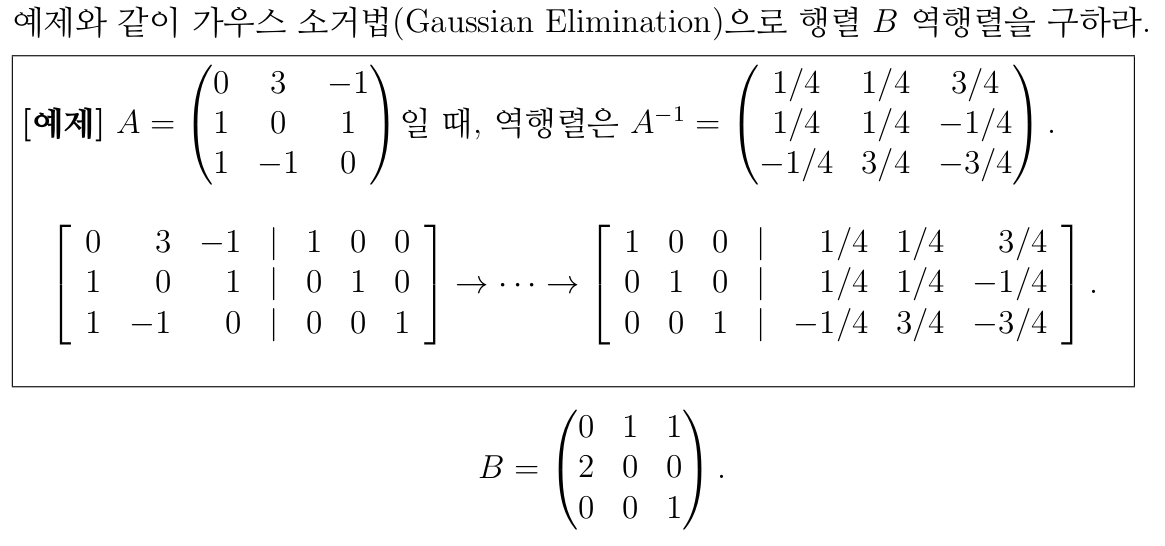
\includegraphics[scale=.35]{asgmt1_2.png}
\end{figure}
\begin{proof}[\sol]
	 Since \begin{align*}
		\left[\begin{array}{ccc|ccc}
			0&1&1 &1&0&0\\
			2&0&0 &0&1&0\\
			0&0&1 &0&0&1
		\end{array}\right]\xrightarrow{\text{Swap $R_1$ and $R_2$}}\left[\begin{array}{ccc|ccc}
		2&0&0 &0&1&0\\
		0&1&1 &1&0&0\\
		0&0&1 &0&0&1
	\end{array}\right]&\rightarrow\left[\begin{array}{ccc|ccc}
	1&0&0 &0&1/2&0\\
	0&1&1 &1&0&0\\
	0&0&1 &0&0&1
\end{array}\right]\quad R_1\gets R_1/2\\
	&\rightarrow\left[\begin{array}{ccc|ccc}
		1&0&0 &0&1/2&0\\
		0&1&0 &1&0&-1\\
		0&0&1 &0&0&1
	\end{array}\right]\quad R_2\gets R_2-R_3,
	\end{align*} we have $$\inv{B}=\begin{pmatrix}
	0&1/2&0\\1&0&-1\\0&0&1
\end{pmatrix}.$$
\end{proof}

\newpage
\item \ \begin{figure}[h!]
	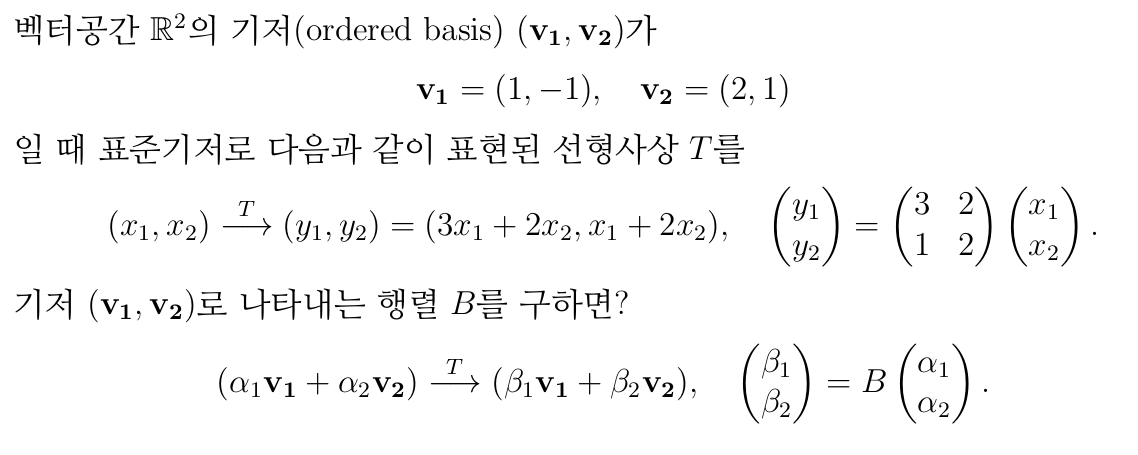
\includegraphics[scale=.35]{asgmt1_3.png}
\end{figure}
\begin{proof}[\sol]
	Note that \begin{center}
		\begin{tikzcd}
			&& \R^2 \arrow[rr, "T"] && \R^2\\
			&& \mathscr{B} \arrow[rr, "A_T"] && \mathscr{B} \arrow[dd, "T=S^{-1}"']\\
			&& &&\\
			&& \tilde{\mathscr{B}} \arrow[uu, "S"] \arrow[rr, "B"] && \tilde{\mathscr{B}}           
		\end{tikzcd}
	\end{center} where $A_T=\begin{bmatrix}
	3&2\\1&2
\end{bmatrix}$, $
	\basis=\begin{bmatrix}
		\textbf{e}_1&\textbf{e}_2
	\end{bmatrix}=\begin{bmatrix}
	1&0\\0&1
\end{bmatrix}\ \text{and}\ \hat{\basis}=\begin{bmatrix}
	\textbf{v}_1&\textbf{v}_2
	\end{bmatrix}=\begin{bmatrix}
	1&2\\-1&1
	\end{bmatrix}.$ Since \[
	\left[\begin{array}{cc|cc}
		1&2 &1&0\\-1&1 &0&1
	\end{array}\right]\rightarrow\left[\begin{array}{cc|cc}
	1&2 &1&0\\0&3 &1&1
\end{array}\right]\rightarrow\left[\begin{array}{cc|cc}
1&2 &1&0\\0&2 &2/3&2/3
\end{array}\right]\rightarrow\left[\begin{array}{cc|cc}
1&0 &1/3&-2/3\\0&2 &2/3&2/3
\end{array}\right]\rightarrow\left[\begin{array}{cc|cc}
1&0 &1/3&-2/3\\0&1 &1/3&1/3,
\end{array}\right]
	\] \begin{align*}
	B=S^{-1}A_TS&=
	\begin{bmatrix} 1&2\\-1&1 \end{bmatrix}
	\begin{bmatrix} 3&2\\1&2 \end{bmatrix}
	\begin{bmatrix} 1/3&-2/3\\1/3&1/3 \end{bmatrix}\\
	&=
	\begin{bmatrix} 5&6\\2&0 \end{bmatrix}
	\begin{bmatrix} 1/3&-2/3\\1/3&1/3 \end{bmatrix}\\
	&=
	\begin{bmatrix} 11/3&-4/3\\2/3&-4/3 \end{bmatrix}.
\end{align*}
\end{proof}
\newpage
\item \ \begin{figure}[h!]
	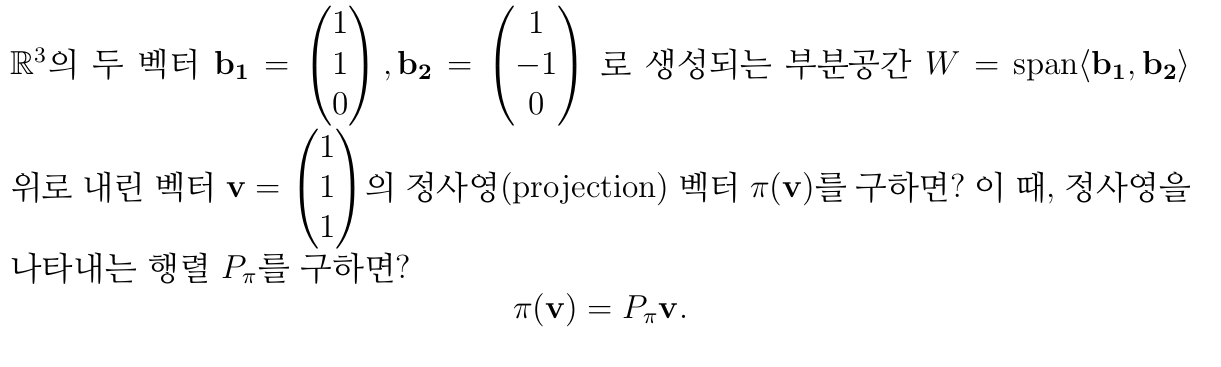
\includegraphics[scale=.35]{asgmt1_4.png}
\end{figure}
\begin{proof}[\sol]
Let $
\textbf{B}=\begin{bmatrix} \textbf{b}_1&\textbf{b}_2\end{bmatrix}
=\begin{bmatrix}
	1&1\\1&-1\\0&0
\end{bmatrix}.$ Since $\textbf{B}^T\textbf{B}=\begin{bmatrix}
1&1&0\\1&-1&0
\end{bmatrix}\begin{bmatrix}
1&1\\1&-1\\0&0
\end{bmatrix}=\begin{bmatrix}
2&0\\0&2
\end{bmatrix}$, we have \[
\left[\begin{array}{cc|cc}
	2&0& 1&0\\
	0&2& 0&1
\end{array}\right]\rightarrow\left[\begin{array}{cc|cc}
1&0 &1/2&0\\
0&1 &0&1/2
\end{array}\right]\implies\inv{(\textbf{B}^T\textbf{B})}=\begin{bmatrix}
1/2&0\\0&1/2
\end{bmatrix}.
\] Then \begin{align*}
	\boldsymbol{\lambda}=\inv{(\textbf{B}^T\textbf{B})}\textbf{B}^T\textbf{v}
	=\begin{bmatrix}
		1/2 &0\\0&1/2
	\end{bmatrix}\begin{bmatrix}
	1&1&0\\1&-1&0
\end{bmatrix}\begin{bmatrix}
	1\\1\\1
\end{bmatrix}=\begin{bmatrix}
1/2&-1/2&0\\ 1/2&1/2&0
\end{bmatrix}\begin{bmatrix}
1\\1\\1
\end{bmatrix}=\begin{bmatrix}
0 \\ 1
\end{bmatrix}.
\end{align*} Thus, \[
\pi_W(\vec{v})=\textbf{B}\boldsymbol{\lambda}
=\begin{bmatrix}
	1&1\\1&-1\\0&0
\end{bmatrix}\begin{bmatrix}
0 \\ 1
\end{bmatrix}=\begin{bmatrix}
1\\-1\\0
\end{bmatrix}
\] and \[
P_\pi=\textbf{B}\inv{(\textbf{B}^T\textbf{B})}\textbf{B}^T
=\begin{bmatrix}
	1&1\\1&-1\\0&0
\end{bmatrix}\begin{bmatrix}
1/2&-1/2&0\\ 1/2&1/2&0	
\end{bmatrix}=\begin{bmatrix}
1&0&0\\0&-1&0\\0&0&0
\end{bmatrix}.
\]
\end{proof}
\newpage
\item \ \begin{figure}[h!]
	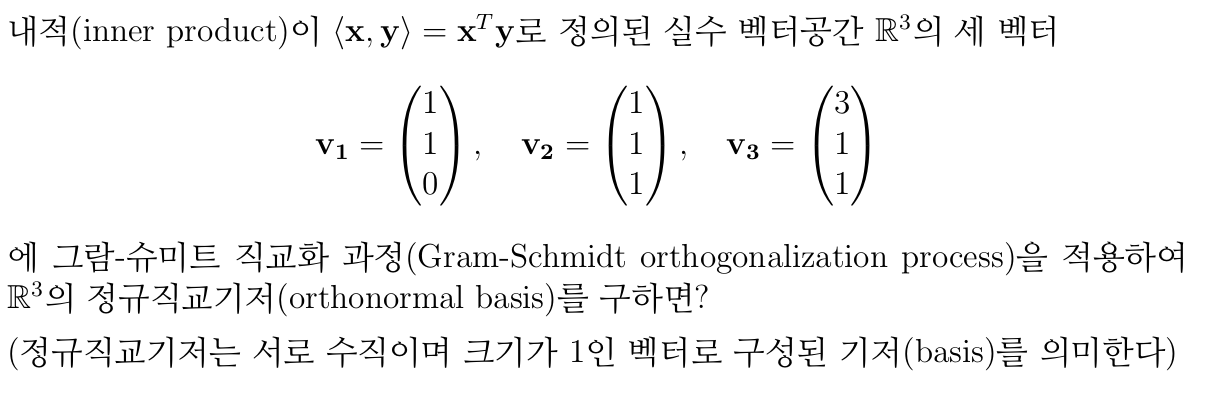
\includegraphics[scale=.35]{asgmt1_5.png}
\end{figure}
\begin{proof}[\sol]
	\begin{enumerate}[(i)]
		\item (1st vector) Let \(\textbf{u}_1:=\textbf{v}_1=\begin{bmatrix}
			1&1&0
		\end{bmatrix}^T.\) Since \(\norms{\vec{u}_1}=\sqrt{1^2+1^2+0^2}=\sqrt{2}\), we have \[
		\textbf{w}_1:=\frac{\vec{u}_1}{\norms{\vec{u}}}=\frac{1}{\sqrt{2}}\begin{bmatrix}
			1\\1\\0
		\end{bmatrix}.
		\]
		\item (2nd vector) \begin{align*}
			\vec{u}_2:=\vec{v}_2-\pi_{\Span{\vec{u}_1}}(\vec{v}_2)=\vec{v}_2-\frac{\vec{u}_1\vec{u}_1^T}{\norms{\vec{u}_1}^2}\vec{v}_2=\begin{bmatrix}
				1\\1\\1
			\end{bmatrix}-\frac{1}{2}\begin{bmatrix}
			1\\1\\0
		\end{bmatrix}\begin{bmatrix}
		1&1&0
	\end{bmatrix}\begin{bmatrix}
	1\\1\\1
\end{bmatrix}
		&=\begin{bmatrix}
			1\\1\\1
		\end{bmatrix}-\frac{1}{2}
		\begin{bmatrix}
			1 & 1 & 0\\ 1& 1 &0\\ 0&0&0
		\end{bmatrix}\begin{bmatrix}
		1\\1\\1
	\end{bmatrix}\\
		&=\begin{bmatrix}
			1\\1\\1
		\end{bmatrix}-\frac{1}{2}
		\begin{bmatrix}
			2 \\2\\0
		\end{bmatrix}=\begin{bmatrix}
		0\\0\\1
	\end{bmatrix}.
		\end{align*} Thus $\displaystyle
		\vec{w}_2:=\frac{\vec{u}_2}{\norms{\vec{u}_2}}=\begin{bmatrix}
			0\\0\\1
		\end{bmatrix}.$
		\item (3rd vector) Let \(\textbf{B}=\begin{bmatrix}
			\textbf{u}_1&\vec{u}_2
		\end{bmatrix}=\begin{bmatrix}
		1&0\\
		1&0\\
		0&1
	\end{bmatrix}\) then \(\textbf{B}^T\textbf{B}=\begin{bmatrix}
	1&1&0\\
	0&0&1
\end{bmatrix}\begin{bmatrix}
1&0\\
1&0\\
0&1
\end{bmatrix}=\begin{bmatrix}
	2&0\\0&1
\end{bmatrix}\) and so \begin{align*}
	\pi_{\Span{\vec{u}_1,\vec{u}_2}}=\textbf{P}_\pi=\textbf{B}(\textbf{B}^T\textbf{B})^{-1}\textbf{B}^T=\begin{bmatrix}
		1&0\\
		1&0\\
		0&1
	\end{bmatrix}\begin{bmatrix}
	1/2&0\\0&1
\end{bmatrix}\begin{bmatrix}
1&1&0\\
0&0&1
\end{bmatrix}
=\begin{bmatrix}
	1/2&0\\1/2&0\\0&1
\end{bmatrix}\begin{bmatrix}
1&1&0\\
0&0&1
\end{bmatrix}=\begin{bmatrix}
1/2&1/2&0\\1/2&1/2&0\\0&0&1
\end{bmatrix}.
\end{align*} Thus,
\begin{align*}
	\vec{u}_3:=\vec{v}_3-\pi_{\Span{\vec{u}_1,\vec{u}_2}}(\vec{v}_3)=\vec{v}_3-\textbf{P}_{\pi}\vec{v}_3=(\textbf{I}_3-\textbf{P}_\pi)\vec{v}_3
	&=\begin{bmatrix}
		1/2&-1/2&0\\-1/2&1/2&0\\0&0&0
	\end{bmatrix}\begin{bmatrix}
	3\\1\\1
\end{bmatrix}=\begin{bmatrix}
1\\-1\\0
\end{bmatrix}
\end{align*} and then $\displaystyle
\textbf{w}_3:=\frac{\vec{u}_3}{\norms{\vec{u}_3}}=\frac{1}{\sqrt{2}}\begin{bmatrix}
	1\\-1\\0
\end{bmatrix}.$
	\end{enumerate}
	By (i),(ii) and (iii), we have orthonormal basis \[
	\set{\textbf{w}_1,\textbf{w}_2,\textbf{w}_3}=\set{\frac{1}{\sqrt{2}}\begin{bmatrix}
			1\\1\\0
	\end{bmatrix},\begin{bmatrix}
	0\\0\\1
\end{bmatrix},\frac{1}{\sqrt{2}}\begin{bmatrix}
1\\-1\\0
\end{bmatrix}}.
	\]
\end{proof}
\vspace{20pt}
\item \ \begin{figure}[h!]
	
\includegraphics[scale=.35]{asgmt1_6.png}
\end{figure}
\begin{proof}[\sol]
\begin{align*}
	{\begin{vmatrix}
		1&x_1&x_1^2\\
		1&x_2&x_2^2\\
		1&x_3&x_3^2
	\end{vmatrix}}&=\begin{vmatrix}
	x_2 & x_2^2\\x_3&x_3^2
\end{vmatrix}-x_1\begin{vmatrix}
	1&x_2^2\\1&x_3^2
\end{vmatrix}+x_1^2\begin{vmatrix}
	1&x_2\\1&x_3
\end{vmatrix}\\
	&=(x_2x_3^2-x_2^2x_3)-x_1(x_3^2-x_2^2)+x_1^2(x_3-x_2)\\
	&=x_2x_3(x_3-x_2)-x_1(x_2+x_3)(x_2-x_3)+x_1^2(x_3-x_2)\\
	&=x_2x_3(x_3-x_2)+x_1(x_2+x_3)(x_3-x_2)+x_1^2(x_3-x_2)\\
	&=x_2x_3(x_3-x_2)+x_1(x_3-x_2)(x_1+x_2+x_3)\\
	&=(x_3-x_2)(x_2x_3+x_1(x_1+x_2+x_3)).
\end{align*}
\end{proof}
\newpage
\item \ \begin{figure}[h!]
	
\includegraphics[scale=.35]{asgmt1_7.png}
\end{figure}
\begin{proof}[\sol]
	\ \begin{enumerate}[(Step 1)]
		\item \textbf{Find the Eigenvalues:} \[
		\det(A-\lambda I_2)=\abs{\begin{matrix}
				2-\lambda& 1\\1&2-\lambda
		\end{matrix}}=(2-\lambda)^2-1=\lambda^2-4\lambda+3=(\lambda-3)(\lambda-1)=0.
		\] Thus, \(\lambda_1:=3\) and $\lambda_2:=1$.
		\item \textbf{Find the Eigenvectors:}
		\begin{enumerate}[(i)]
			\item For $\lambda_1=3$, \[
			\begin{bmatrix}
				-1&1\\1&-1
			\end{bmatrix}\begin{bmatrix}
			x_1\\x_2
		\end{bmatrix}=\begin{bmatrix}
		0\\0
	\end{bmatrix}\implies\vec{v}_1:=\begin{bmatrix}
	1\\1
\end{bmatrix}.
			\]
			\item For $\lambda_2=1$, \[
			\begin{bmatrix}
				1&1\\1&1
			\end{bmatrix}\begin{bmatrix}
				x_1\\x_2
			\end{bmatrix}=\begin{bmatrix}
				0\\0
			\end{bmatrix}\implies\vec{v}_2:=\begin{bmatrix}
				1\\-1
			\end{bmatrix}.
			\]
		\end{enumerate}
		\item \textbf{Normalize the Eigenvectors:} \[
		\hat{\vec{v}}_1:=\frac{1}{\sqrt{2}}\begin{bmatrix}
			1\\1
		\end{bmatrix}=\begin{bmatrix}
		1/\sqrt{2}\\1/\sqrt{2}
	\end{bmatrix},\quad\hat{\vec{v}}_2:=\frac{1}{\sqrt{2}}\begin{bmatrix}
	1\\-1
\end{bmatrix}=\begin{bmatrix}
1/\sqrt{2}\\-1/\sqrt{2}
\end{bmatrix}.
		\]
		\item \textbf{Construct $P$ and $D$:} \begin{align*}
			&P:=\begin{bmatrix}
				\hat{\vec{v}}_1&\hat{\vec{v}}_2
			\end{bmatrix}=\begin{bmatrix}
			1/\sqrt{2}&1/\sqrt{2}\\1/\sqrt{2}&-1/\sqrt{2}
		\end{bmatrix},\\
		&D:=\begin{bmatrix}
			\lambda_1&0\\0&\lambda_2
		\end{bmatrix}=\begin{bmatrix}
		3&0\\0&1
	\end{bmatrix}.
		\end{align*}
	\end{enumerate}
	By Step 1-4, hence, \[
	A=PDP^T=\begin{bmatrix}
		\frac{1}{\sqrt{2}}&\frac{1}{\sqrt{2}}\\
		\frac{1}{\sqrt{2}}&-\frac{1}{\sqrt{2}}
	\end{bmatrix}\begin{bmatrix}
	3&0\\0&1
\end{bmatrix}\begin{bmatrix}
\frac{1}{\sqrt{2}}&\frac{1}{\sqrt{2}}\\
\frac{1}{\sqrt{2}}&-\frac{1}{\sqrt{2}}
\end{bmatrix}.
	\]
\end{proof}
\newpage
\item \ \begin{figure}[h!]
	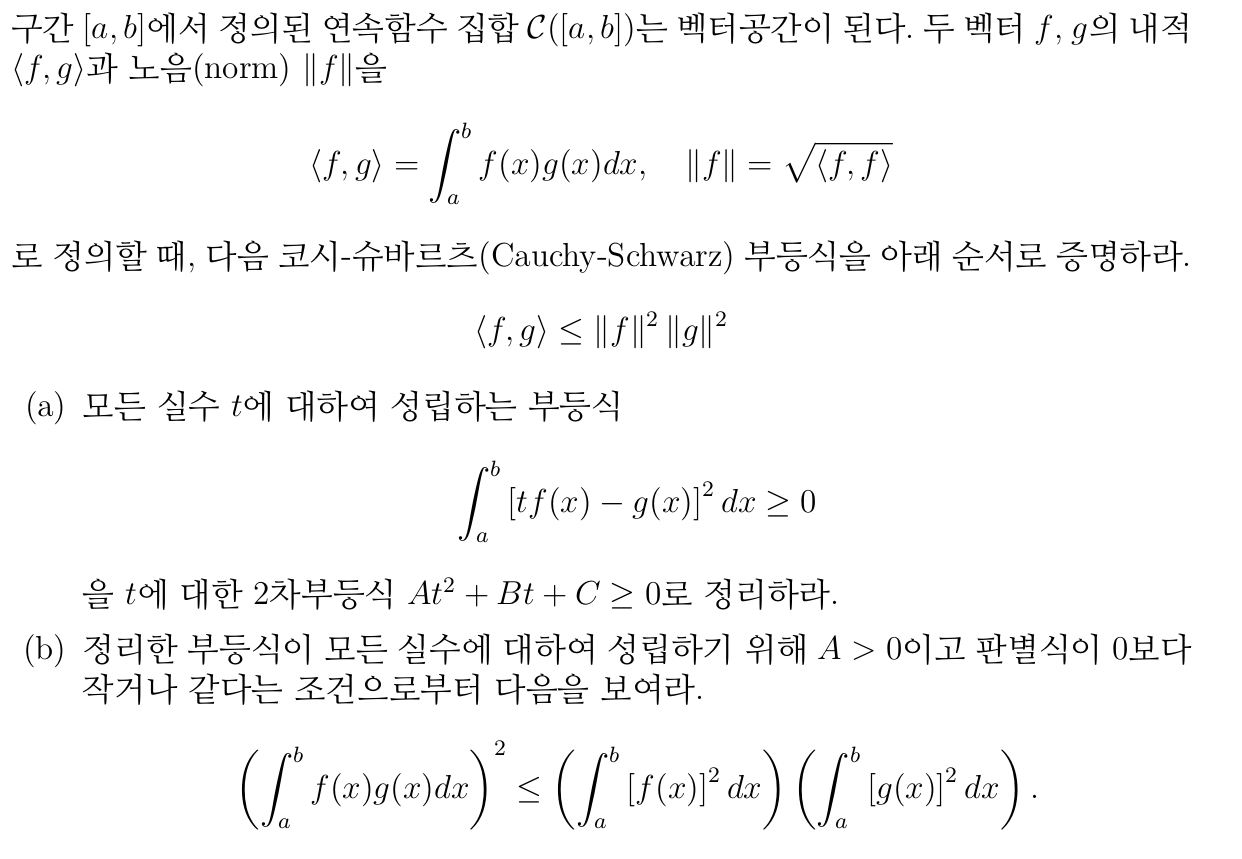
\includegraphics[scale=.325]{asgmt1_8.png}
\end{figure}
\begin{proof}[\sol]
\begin{enumerate}[(a)]
	\item \begin{align*}
		\int_a^b\sbr{tf(x)-g(x)}^2\ dx\geq0 &\iff \int_a^b\sbr{t^2[f(x)]^2-2tf(x)g(x)+[g(x)]^2}\ dx \geq 0\\
		&\iff t^2\int_a^b[f(x)]^2\ dx-2t\int_a^bf(x)g(x)\ dx+\int_a^b[g(x)]^2\ dx\geq 0\\
		&\iff At^2+Bt+C\geq0\quad\text{with}\quad\begin{cases}
			A=\int_a^b[f(x)]^2\ dx,\\
			B=-2\int_a^bf(x)g(x)\ dx,\\
			C=\int_a^b[g(x)]^2\ dx.
		\end{cases}
	\end{align*}
	\item \begin{align*}
		&B^2-4AC=\del{-2\int_a^bf(x)g(x)\ dx}^2-4\del{\int_a^b[f(x)]^2\ dx}\del{\int_a^b[g(x)]^2\ dx}\leq 0\\
		\implies&
		4\del{\int_a^bf(x)g(x)}\leq 4\del{\int_a^b[f(x)]^2\ dx}\del{\int_a^b[g(x)]^2\ dx}\\
		\implies&\left(\int_a^bf(x)g(x)\ dx\right)^2\leq\left(\int_a^b[f(x)]^2\ dx\right)\left(\int_a^b[g(x)]^2\ dx\right).
	\end{align*}
\end{enumerate}
\end{proof}
\newpage
\item \ \begin{figure}[h!]
	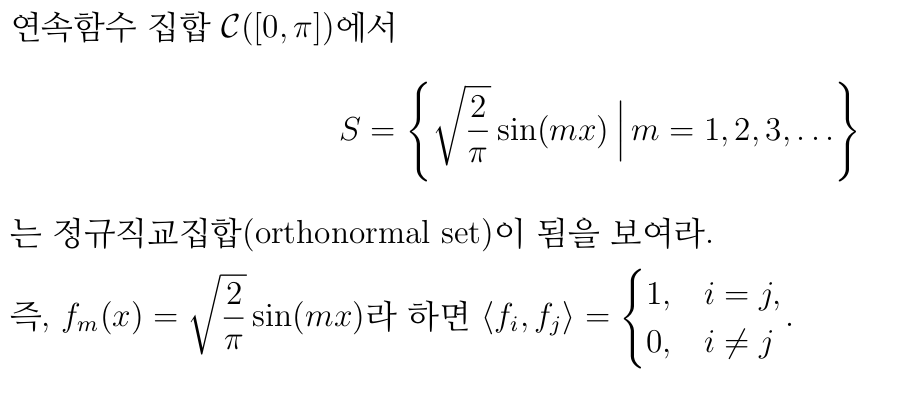
\includegraphics[scale=.35]{asgmt1_9.png}
\end{figure}
\begin{proof}[\sol]
\begin{enumerate}[(i)]
	\item \textbf{Normalization.} We want to show that \[
	\norms{f_m}^2=\inner{f_m,f_m}=\int_0^\pi [f_m(x)]^2\ dx=1.
	\] Now, we have \begin{align*}
		\int_0^\pi [f_m(x)]^2\ dx=\int_0^\pi\del{\sqrt{\frac{2}{\pi}}\sin(mx)}^2\ dx&=\frac{2}{\pi}\int_0^\pi\sin^2(mx)\ dx\\
		&=\frac{2}{\pi}\int_0^\pi\frac{1-\cos(2mx)}{2}\ dx\\
		&=\frac{2}{\pi}\int_0^\pi\del{\frac{1}{2}-\frac{1}{2}\cos(2mx)}\ dx\\
		&=\frac{2}{\pi}\sbr{\frac{1}{2}x-\frac{1}{4m}\sin(2mx)}_0^\pi\\
		&=\frac{2}{\pi}\sbr{\frac{\pi}{2}-0-(0-0)}\\
		&=1.
	\end{align*}
	\item \textbf{Orthogonality.} Let \(m\neq n\). We want to show that \[
	\inner{f_m,f_n}=\int_0^\pi f_m(x)f_n(x)\ dx = 0.
	\] Now, we have \begin{align*}
		\int_0^\pi f_m(x)f_n(x)\ dx&=\int_0^\pi\sqrt{\frac{2}{\pi}}\sin(mx)\sqrt{\frac{2}{\pi}}\sin(nx)\ dx\\
		&=\frac{2}{\pi}\int_0^\pi\sin(mx)\sin(nx)\ dx.
	\end{align*} Since $\sin x\sin y=\frac{1}{2}\del{\cos(x-y)-\cos(x+y)}$, we obtain \[
	\int_0^\pi f_m(x)f_n(x)\ dx=\frac{1}{\pi}\int_0^\pi\cos((m-n)x)\ dx-\frac{1}{\pi}\int_0^\pi\cos((m+n)x)\ dx.
	\] Since integrating cosine function over a whole period result in \(0\), thus, \[
	\int_0^\pi f_m(x)f_n(x)=0.
	\] Therefore, any two different element in \(S\) are orthogonal each other.
\end{enumerate}
\end{proof}
\end{enumerate}




\footer{Department of Information Security, Cryptology and Mathematics
\\ College of Science and Technology
\\ Kookmin University}
\end{document}